\chapter{Requirements and Specifications} \label{ch:reqandspec}

As mentioned in section \ref{ch:introduction:sec:project_aims}, the overall goal of the application is to build a web application where teachers can create SQL assignments and students can submit solutions which are automatically graded. Therefore, the requirements of the project can be split in two parts: the requirements for the web application, and the requirements for the grading algorithm.

\section{Requirements} \label{ch:reqandspec:sec:rec}

\subsection{Web application}
\begin{enumerate}[label=R-\arabic*]
  \item The web application should be able to store data in a database
  \item The web application should allow users to log-in and keep their data
    across sessions.
  \item The web application should allow users to have different roles within the
    application (e.g. Student/ Teacher/ TA)
  \item  A teacher should be able to create assignments by giving a title, a description, and a SQL query that creates the tables and the relations between them, a SQL query that seeds the table with initial data, and a SQL query which represents the correct answer for the assignment.
  \item The application should compile the queries provided and if no errors are shown, it will save the assignment in the database and display the schema of the database and the data from it.
  \item The teacher should allow editing the assignments after they are created.
  \item The teacher should allow the deletion assignments after they are created.
  \item A student should be able to provide solutions to assignments by submitting a SQL query. The web application should return the results instantly to the students after it assess the query. If any compilation errors are returned, they will be shown to the student.
  \item A student should be able to view the schema of the database for the assignment.
  \item A student should be able to see hints if they make any errors, or they can also see a breakdown of the components from the teacher's query and the ones used by their query.
  \item SQL typing on the web application should be made in a browser based code editor that provides syntax highlighting.
  \item Teachers should be able to have a graphical view of the results and download the results in a CSV format. In addition, they should be able to view the results of individual submissions.
\end{enumerate}

\subsection{Grading SQL library}
\begin{enumerate}[label=G-\arabic*]
  \item The library should be able to connect to a \text{MySQL} server and execute queries on a given database.
  \item The library should handle any error that might occur when communicating to the database (including failed execution of SQL queries, connection issues, etc.) and not throw an un-handled error.
  \item The libary should prevent the use of SQL injection and any potential data leak from the database.
  \item The library should expose a method that allows the compilation of an assignment given a schema query, a seed query and a correct query. The application should return the schema and the data of the database if no errors are encountered. If errors are encountered, then it should return the appropriate error.
  \item The library should be able to canonicalize a query using the transformations described in section \ref{ch:lit:sec:improved_canon}.
  \item The library can compare the results of two SQL queries and check if they match.
  \item The library should be able to grade a student's SQL submission by comparing to the instructor's SQL after canonicalizing and applying the grading algorithm in \ref{ch:lit:sec:improved_grading}.
  \item The library should provide a detailed grade which contains the grade of each component.
  \item The library should provide hints about fixing the student's query if the two queries are different.
  \item The library should clear all tables and data from a database after the compilation of any assignment or the assessment of a submission.
\end{enumerate}

\section{Specifications} \label{ch:reqandspec:sec:spec}

These requirements can easily be implemented in a multitude of languages and frameworks as there are no language or framework specific requirements. For this project, we have opted to build this in the Ruby programming language using two applications:
\begin{enumerate}
    \item A Ruby library (or gem as it's called in Ruby) that will handle the requirements related to the grading of queries.
    \item A Ruby on Rails application that will handle the requirements related to the web application.
\end{enumerate}

The decision to split the application in two separate components was made in order to separate the concerns and to allow for independent work to happen on each application. Furthermore, by separating the library from the main web application we gain the ability use the library in other use cases (e.g. for building a Command-Line Interface). It also means that the library does not care about how the grades are displayed, or how the exercises and submissions are stored in the database.

Finally, by using a separate library, we can make use of encapsulation - hiding away the implementation details of grading from the web application which is only meant to work with final results.

We have opted for a Ruby programming language based on the following criteria:

\begin{itemize}
    \item Past experience with the programming language and the associated framework means that more time could be spent on the grading algorithm, rather than learning a new language and a new framework.
    \item Ruby has database driver for all popular databases. That means that in the future this application could be extended to run not only MySQL queries, but also other formats of queries. \footnote{While most queries use standard SQL, each database adds its own features which can make the queries incompatible with each other.}
    \item Ruby on Rails is one of the most popular and easy to use web application framework. It is a very opinionated framework which means it allowed us less time deciding on which way to implement certain features.
\end{itemize}

\subsection{Development process}

Although the two libraries allow parallel development, throughout the development of the project a waterfall approach will be used. The general pattern of development is the following:

\begin{enumerate}
  \item Implement and test feature in library and publish new version of the library
  \item Update web application to the last version of library
  \item Update the web application existing code and test if any interfaces were changed
  \item Implement and test new features in the web application.
\end{enumerate}

All new features added in library and the web application will be tested at the time of development. To ensure this, three tools are used:
\begin{itemize}
  \item \textbf{Git \& Github Pull requests (PR)}: development will be done using the Git Version Control System. All new features will be developed on a separate branch than master, and to get them in master a new PR will be submitted on GitHub.
  \item \textbf{Travis} is a continuous integration system that will execute all tests from any Git commit. This will ensure that all features added are working according to the tests, and that existing features are not affected by the new changes.
  \item \textbf{Codecov} is a tool that counts the code coverage of code from a PR. Whenever a new commit is pushed to a PR, codecov's code coverage is recalculated and a message is left on the PR.
\end{itemize}
Both Travis and CodeCoverage, will provide \textit{checks} on Github PRs that are required for a PR to be merged.

\begin{figure}[h]
    \centering
    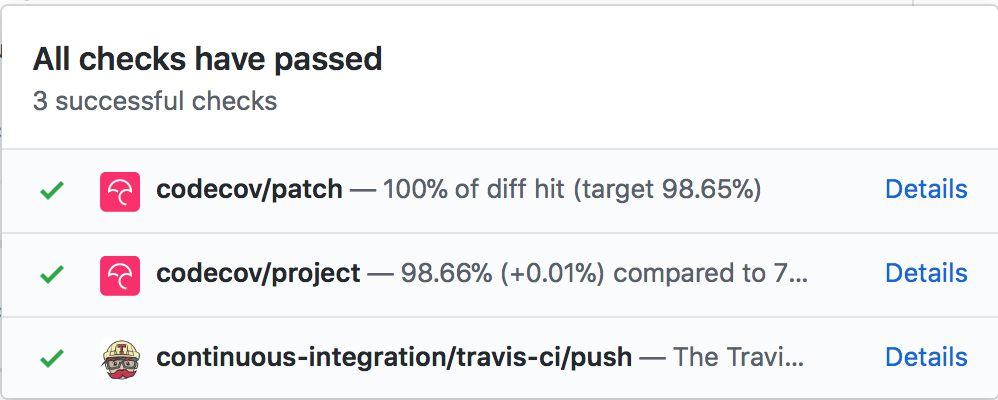
\includegraphics[width=(\linewidth / 3 * 2)]{Chapters/3-RequirementAndSpecifications/github_checks.png}
    \caption{Example of GitHub PR checks}
    \label{fig:create_assignment}
\end{figure}

\subsection{Platform dependencies}

The application (including the library) has only two dependencies:
\begin{itemize}
    \item A MySQL server
    \item The ability to run Ruby (and Ruby on Rails)
\end{itemize}

\subsection{Specifications for the web application}

\begin{tabularx}{\textwidth}{|c|Y|Y|}
  \hline
  \textbf{R no.} & \textbf{Requirement details} & \textbf{Specification} \\\hline
  \endhead
  R-1 & The web application should be able to store data in a database & Use ActiveRecord to store and access data in a MySQL server \\\hline
  R-2 & The web application should allow users to log-in and keep their data across sessions. & Use devise library for authentication \\\hline
  R-3 &  The web application should allow users to have different roles within the application (e.g.Student/ Teacher/ TA) & Use pundit library for user roles management \\\hline
  R-4 &  A teacher should be able to create assignments by giving a title, a description, and a SQL query that creates the tables and the relations between them, a SQL query that seeds the table with initial data, and a SQL query which represents the correct answer for the assignment. & Provide a web form built in Bootstrap that provides a code editor using codemirror \\\hline
  R-5 &  The application should compile the queries provided and if no errors are shown, it will save the assignment in the database and display the schema of the database and the data from it. & Use the compile method provide by the library and defined and display any error that may occur, otherwise save the record in the database. \\\hline
  R-6 & The teacher should allow editing the assignments after they are created. & Updates the card in the database and re-compiles the query. \\\hline
  R-7 & The teacher should allow the deletion assignments after they are created. & Deletes the challenge from database \\\hline
  R-8 & A student should be able to provide solutions to assignments by submitting a SQL query. The web application should return the results instantly to the students after it assess the query. If any compilation errors are returned, they will be shown to the student. & Provide a web form built in Bootstrap that provides a code editor using codemirror. Assess the query using the assess method provided by grading library. Save all submissions in the database after they have been assessed. \\\hline
  R-9 & A student should be able to view the schema of the database for the assignment. & Render a HTML views that contains the schema of the database and provide a form written in Bootstrap and codemirror where they provide solutions. \\\hline
  R-10 & A  student  should  be  able  to  see  hints  if  they  make  any  errors,  or  they  can  also  see  a breakdown of the components from the teacher’s query and the ones used by their query. & Display a HTML view based on the results of their submission, after being graded. \\\hline
  R-11 & SQL typing on the web application should be made in a browser based code editor that provides syntax highlighting. & Provide a code editor written in codemirror. \\\hline
  R-12 & Teachers should be able to have a graphical view of the results and download the results in  a CSV format.   In  addition,  they  should  be  able  to  view  the  results  of  individual submissions. & Provide a download button that gets the best submission of each student for a certain assignment.. \\\hline
\end{tabularx}

\subsection{Specification for Library}

\begin{tabularx}{\textwidth}{|c|Y|Y|}
  \hline
  \textbf{R no.} & \textbf{Requirement details} & \textbf{Specification} \\\hline
  \endhead
G- & The library should be able to connect to a MySQL server and execute queries on a given database. & Connect to a MySQL database using Ruby library mysql2 \\\hline
G- & The library should handle any error that might occur when communicating to the database (including failed execution of SQL queries, connection issues, etc.) and not throw an un-handled error. & Handle errors returned by mysql2 \\\hline
G- & The libary should prevent the use of SQL injection and any potential data leak from the database. & .\\\hline
G- & The library should expose a method that allows the compilation of an assignment given a schema query, a seed query and a correct query. The application should return the schema and the data of the database if no errors are encountered. If errors are encountered, then it should return the appropriate error. & .\\\hline
G- & The library should be able to canonicalize a query using the transformations described in section \ref{ch:lit:sec:improved_canon}. & .\\\hline
G- & The library can compare the results of two SQL queries and check if they match. & .\\\hline
G- & The library should be able to grade a student's SQL submission by comparing to the instructor's SQL after canonicalizing and applying the grading algorithm in \ref{ch:lit:sec:improved_grading}. & .\\\hline
G- & The library should provide a detailed grade which contains the grade of each component. & .\\\hline
G- & The library should provide hints about fixing the student's query if the two queries are different. & .\\\hline
G- & The library should clear all tables and data from a database after the compilation of any assignment or the assessment of a submission. & .\\\hline
\end{tabularx}
